\documentclass{beamer}

\usepackage{natbib}

\usepackage[frenchb]{babel}

\usepackage[T1]{fontenc}

\usepackage[utf8]{inputenc}

\usepackage{amsmath}

\usepackage[labelformat=empty]{caption}

\usepackage{cclicenses}

\usetheme{Darmstadt}

\title{Le tracking sur le web}

\author{\cc Ilan 'trog' Dubois}

\AtBeginSection[]
{
    \begin{frame}
        \frametitle{Sommaire}
            \tableofcontents[currentsection]
    \end{frame}
}

\begin{document}
    \begin{frame}
        \titlepage
    \end{frame}
    \section{Fonctionnement du tracking}
    \subsection{Les raisons du tracking}
        \begin{frame}
            \begin{center}
                
\includegraphics[scale=0.75]{img/money.jpg}
            \end{center}
        \end{frame}
        \begin{frame}{label=publicite}
            \frametitle{La publicité}
            \begin{center}
                \begin{itemize}
                    \item Les annonceurs publicitaires sont très intéressés par ces techniques.
                    \pause
                    \item Elles permettent en effet de n'envoyer que des annonces qui ont de fortes chances de vous intéresser.
                    \pause
                    \item Le profilage et donc là pour optimiser les dépenses et augmenter l'intérêt des potentiels clients.
                \end{itemize}
            \end{center}
        \end{frame}
        \begin{frame}{label=surveillance}
            \frametitle{La surveillance}
            \begin{center}
                \begin{itemize}
                    \item Ces données peuvent également être utilisées pour effectuer une surveillance des internautes.
                    \pause
                    \item En profilant un utilisateur, on peut prévoir son comportement (avec de très importantes marges d'erreur).
                    \pause
                    \item Dans le cadre de la loi renseignement, les annonceurs peuvent potentiellement avoir à fournir votre historique aux ``boîtes noires``.
                \end{itemize}
            \end{center}
        \end{frame}
    \subsection{Techniques conventionnelles}
        \begin{frame}
            \begin{center}
                \begin{figure}
                    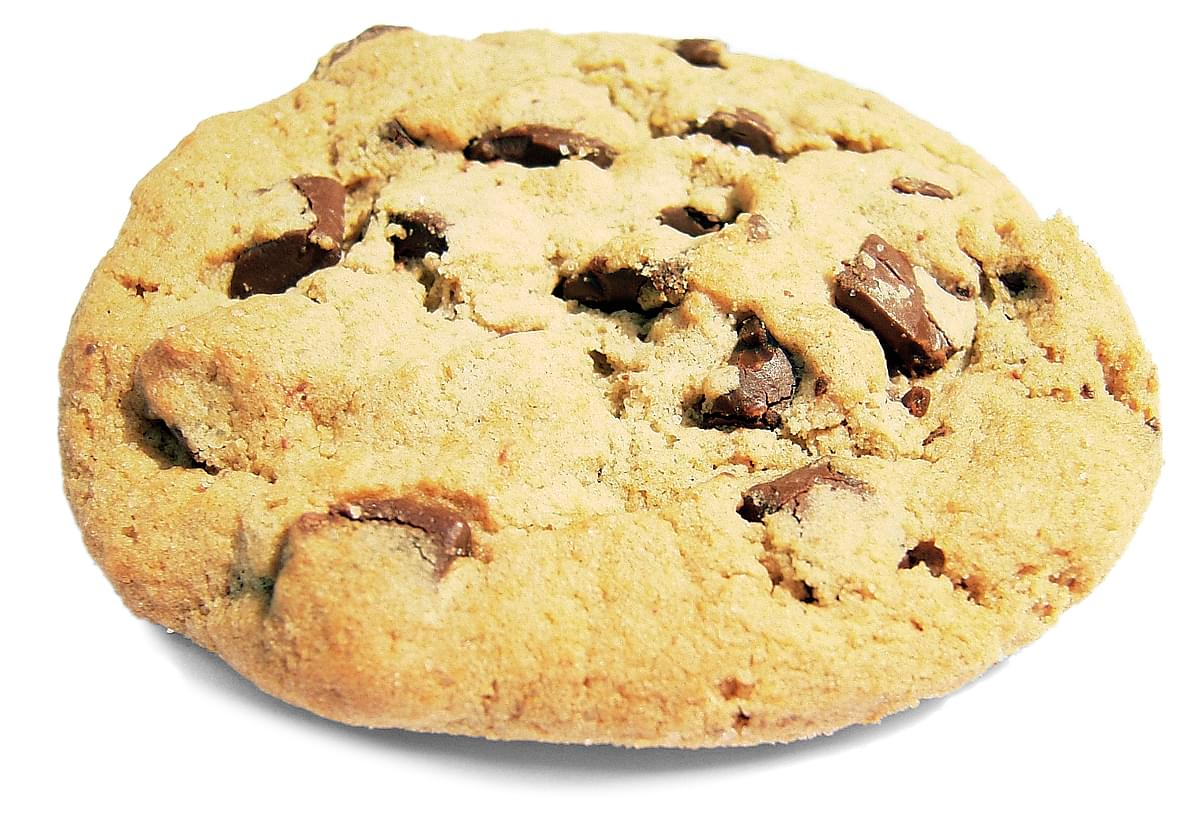
\includegraphics[scale=0.15]{img/cookie.jpg}
                    \caption{\cc --- Bob Smith}
                \end{figure}
            \end{center}
        \end{frame}
        \begin{frame}{label=cookies}
            \frametitle{Les cookies}
            \begin{center}
                \begin{itemize}
                    \item Mini text stocké dans votre navigateur ne pouvant être lu que par le site qui l'a déposé.
                    \item En y laissant un identifiant un site peut facilement vous reconnaître lors de vos visites et reconstituer votre historique sur ce site.
                    \item Les annonceurs utilisent cette pratique pour tracker à l'échelle de plusieurs sites, ce sont des tierces parties.
                \end{itemize}
            \end{center}
        \end{frame}
        \begin{frame}{label=statistiques}
            \frametitle{Les statistiques}
            \begin{center}
                \begin{itemize}
                    \item Pour connaître son audience, un site doit collecter des informations techniques diverses.
                    \item Google avec son service Analytics est très largement utilisé (54\%) pour collecter ces données.
                    \item Ce qui implique que toutes les visites effectuées sur ces sites sont aussi connues de Google.
                \end{itemize}
            \end{center}
        \end{frame}
        \begin{frame}{label=boutons}
            \frametitle{Les boutons de partage}
            \begin{center}
                \begin{itemize}
                    \item Les réseaux sociaux proposent souvent des boutons pour partager le contenu d'une page.
                    \item Lors du chargement du bouton sur la page, celui-ci collecte également des statistiques sur votre visite.
                    \item Les sites comme Facebook ou Twitter peuvent ainsi reconstituer une part très importante de votre historique.
                \end{itemize}
            \end{center}
        \end{frame}
    \subsection{Nouvelles techniques}
        \begin{frame}
            \begin{center}
                \begin{figure}
                    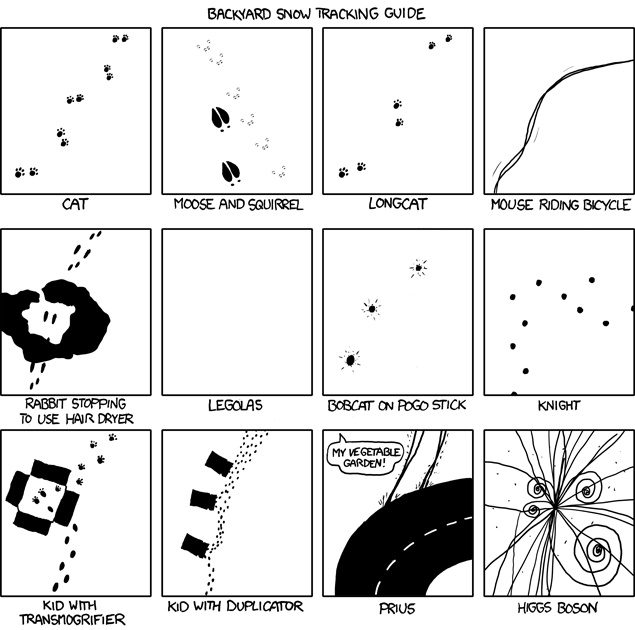
\includegraphics[scale=0.35]{img/snow_tracking.png}
                    \caption{\cc --- xkcd}
                \end{figure}
            \end{center}
        \end{frame}
        \begin{frame}{label=fingerprinting}
            \frametitle{Le fingerprinting}
            \begin{center}
                \begin{itemize}
                    \item La défense contre les systèmes évqués précédemment étant trop aisée pour l'utilisateur, les trackers ont développé de nouvelles techniques \cite{web}.
                    \item Le fingerprinting consiste à vous identifier de façon uniqe avec à votre configuration (matérielle et logiciel) \cite{unique}.
                    \item Pour se défendre, ces systèmes reprennent souvent des fonctionnalités légitimes afin de ne pas être bloquées par l'utilisateur \cite{canvas}.
                    \item L'une de ces méthodes consiste a générer des images particulières tel que son rendu sera dépendant de votre système: Canvas fingerprinting \cite{canvas}.
                \end{itemize}
            \end{center}
        \end{frame}
        \begin{frame}{label=evercookies}
            \frametitle{Ever cookies}
            \begin{center}
                \begin{itemize}
                    \item Les cookies étant \textit{trop} facilement contrôlables, les trackers développent des techniques plus ou moins évoluées pour qu'ils restent \cite{web}.
                    \item Augmenter la durée de vie, utiliser les cookies Flash, respawn les cookies entre eux \cite{web}, dissimuler leur nature...
                    \item Do Not Track réduit de 2,6\% la synchronisation \cite{web}.
                    \item Seul le Tor browser est efficace à 100\% contre les ever cookies
                \end{itemize}
            \end{center}
        \end{frame}
        \begin{frame}{label=partage}
            \frametitle{Partage d'informations (Top 3000 Alexa --- 2014)}
            \begin{center}
                \begin{itemize}
                    \item Le nombre de domaines capables de recouvrir plus de 40\% de l'historique en se basant sur des cookies de tout type est de \textbf{2} \cite{web}.
                    \item En partageant leurs informations ce chiffre passe à \textbf{161} selon estimation modeste (partage avec un unique tracker à la fois) \cite{web}.
                    \item Cette pratique permet à un grand nombre d'entreprises d'avoir un accès conséquent à votre historique.
                \end{itemize}
            \end{center}
        \end{frame}
        \begin{frame}{label=hardware}
            \frametitle{Hardware fingerprinting}
            \begin{center}
                \begin{itemize}
                    \item Toutes les méthodes evoquées précédement sont basées sur des spécificités logiciel de nos machines, et sont donc potentiellement contournables.
                    \item Avec un tracking basé sur les informations materielles, il est en théorie impossible de mentir et donc impossible de fausser ce profilage \cite{hardware}.
                    \item Ces techniques consistent a détécter des irrégularités commises à la fabrication de votre matériel comme d'infimes différences de latence, propres a votre GPU \cite{hardware}.
                    \item Ces techniques sont donc plus difficiles à repousser mais aussi à mettre en place et à fiabiliser pour les trackers, nous ne verrons donc ici pas ce cas.
                \end{itemize}
            \end{center}
        \end{frame}
    \section{Se défendre}
    \subsection{Environnement}
        \begin{frame}
            \begin{center}
                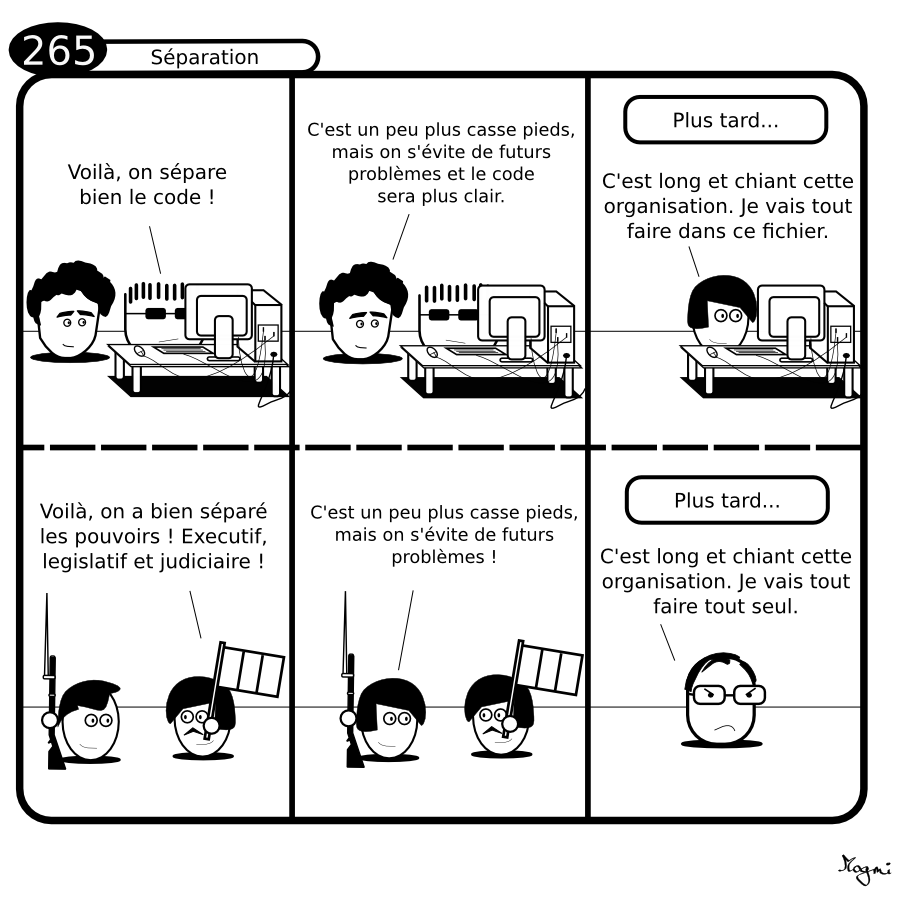
\includegraphics[scale=0.33]{img/265-separation.png}
            \end{center}
        \end{frame}
        \begin{frame}{label=updates}
            \frametitle{Les mises à jour}
            \begin{center}
                \begin{itemize}
                    \item Un environnement de travail à jour améliore la sécurité générale de votre système.
                    \item Il vous permet d'avoir des numéros de version plus communes, donc moins facilement identifiables pour un nouveau tracker \cite{unique}.
                    \item Ne pas oublier d'ajouter l'option \textit{Do No Track}.
                \end{itemize}
            \end{center}
        \end{frame}
        \begin{frame}{label=browser}
            \frametitle{Le navigateur}
            \framesubtitle{Votre navigateur sera votre meilleur allié ou pire ennemi}
            \begin{center}
                \textbf{Chrome, IE, Firefox, Opera\ldots Ces navigateurs ne sont pas égaux!}

                $\displaystyle \begin{bmatrix}
                    \text{Firefox et Chromium sont libres}\\
                    \text{Chromium = Google}\\
                    \text{Firefox = Mozilla}
                \end{bmatrix} \implies 
\includegraphics[scale=0.4]{img/firefox.png}$
            \end{center}
        \end{frame}
    \subsection{Plugins}
        \begin{frame}
            \begin{center}
                \begin{figure}
                    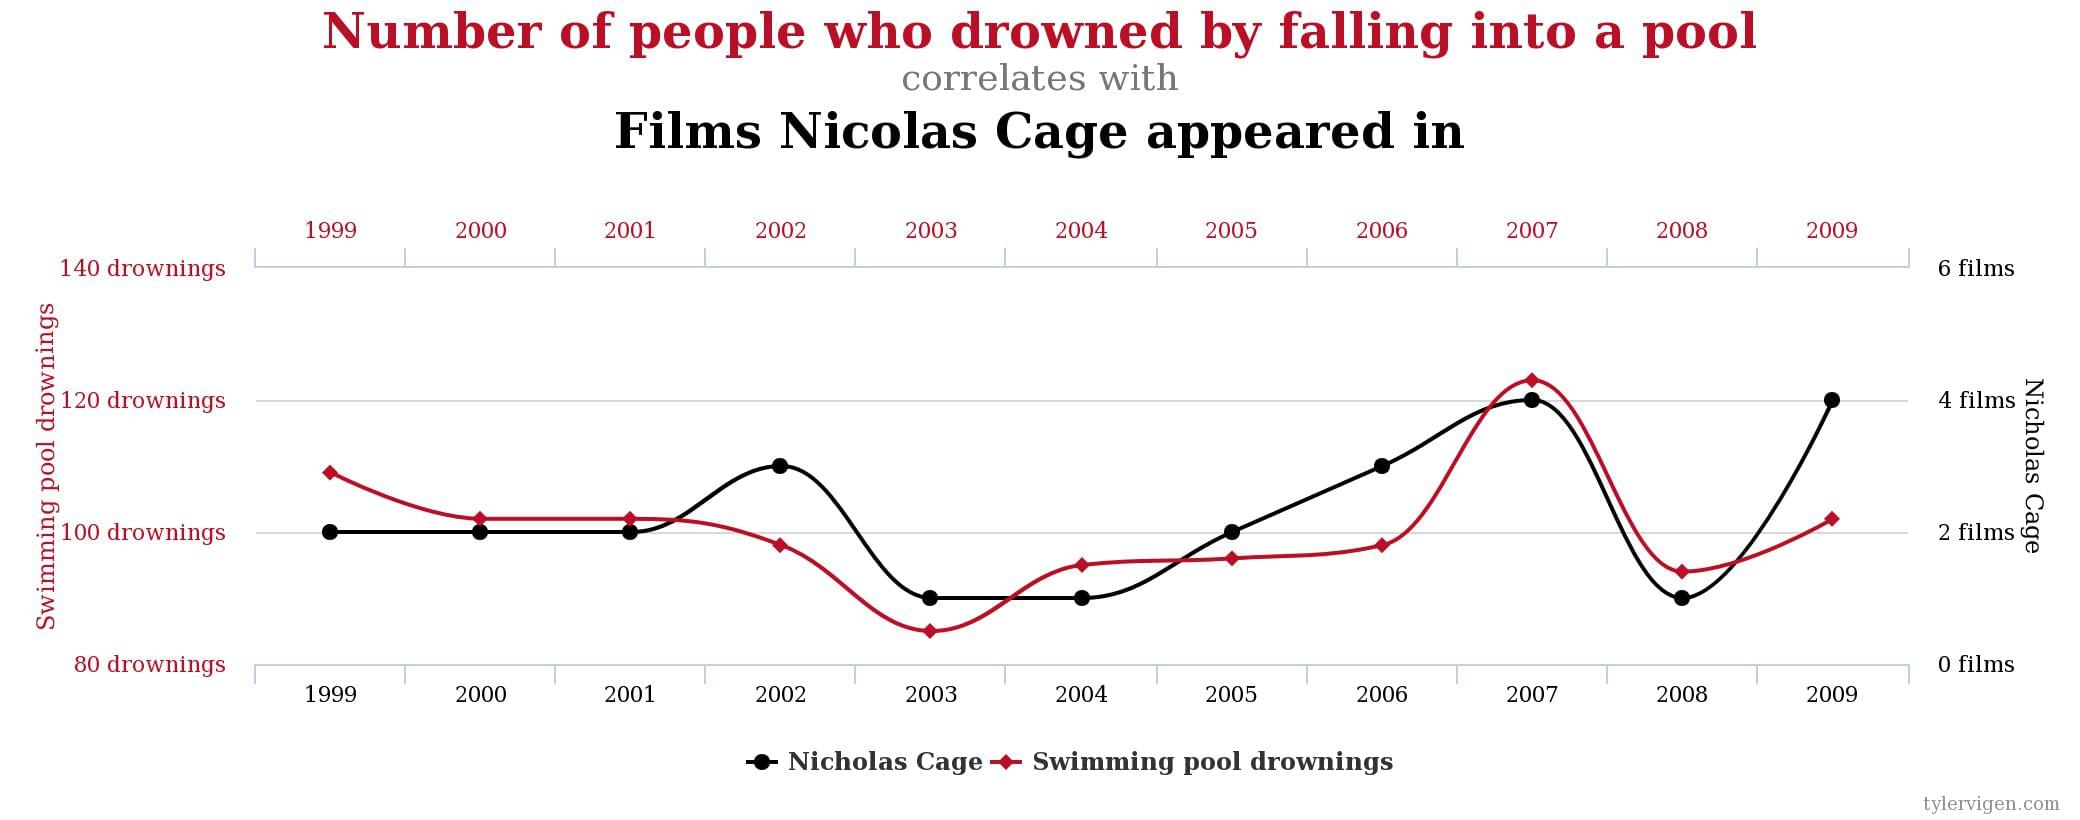
\includegraphics[scale=0.15]{img/data_science.jpg}
                    \caption{\cc --- Tyler Vigen}
                \end{figure}
            \end{center}
        \end{frame}
        \begin{frame}{label=badger}
            \frametitle{Privacy Badger}
            \begin{center}
                \begin{itemize}
                    \item Privacy Badger filtre selon 3 niveux les cookies que les sites mettent sur votre machine.
                    \item Vert c'est OK :)
                    \item Orange le cookie sera bloqué, mais pas le domaine ayant fait la requête.
                    \item Rouge faut plus passer. Le domaine est tout simplement bloqué.
                    \item La configuration standard est tout à fait satisfaisante.
                \end{itemize}
            \end{center}
        \end{frame}
        \begin{frame}{label=adblocker}
            \frametitle{AdBlock}
            \begin{center}
                \begin{itemize}
                    \item Bien qu'il soit de plus en plus contreversé, AdBlock est fiable pour la vie privée.
                    \item A la condition d'utiliser à minima les listes easy list + liste de vos langues + easy privacy.
                    \item Dé-cocher l'autorisation pour certaines publicités.
                    \item La liste easy privacy bloque les trackers de statistiques, les boutons like,\ldots
                \end{itemize}
            \end{center}
        \end{frame}
        \begin{frame}{label=ras}
            \frametitle{Random Agent Spoofer}
            \begin{center}
                \begin{itemize}
                    \item Ce plugin permet de mentir aux trackers quant aux spécificités de votre systeme (versions, programmes)\ldots
                    \item Configurer a Random \textbf{desktop} et \textbf{sans} changement périodique. Exclure dans la liste les navigateurs trop vieux ou exotiques.
                    \item Dans \textit{Headers} cocher Enable DNT et les trois dernières.
                    \item Pour le reste je vous propose de voir mes options et de choisir selon votre convenance.
                \end{itemize}
            \end{center}
        \end{frame}
        \appendix
        \begin{frame}
            \bibliography{src/tracking}{}
            \bibliographystyle{plain}
        \end{frame}
\end{document}
